\subsection{Correctness}
\label{correctness}
In this software abstraction level in our taxonomy, the suggested code by \cct{} should not only be syntactically correct but also solves the task. 
This level does not require \cct{} to suggest the optimal solution for the task but to be able to suggest a solution to a task.
For example, consider a task of perform a sorting operation on a list of numbers. To satisfy this level of abstraction, \cct{} should suggest a syntactically correct list sorting code, which is not required to to be the best algorithm to be the most efficient way.
Figure~\ref{fig:correctness} shows the example and the suggestions from \cct{} at this abstraction level.

\begin{figure}[hbt!]
    \centering
    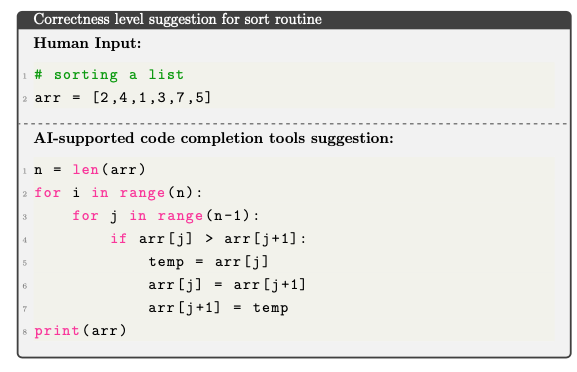
\includegraphics[width=.9\linewidth]{Figures/correctness.png}
    \caption{\cct{} correctness level suggestions}
    \label{fig:correctness}
\end{figure}

The goal of this software abstraction level in our taxonomy is for a \cct{} to be able to suggest a solution rather suggesting the best solution.
The capabilities required by \cct{} to satisfy this level of abstraction are as follows:

\begin{enumerate}
    \item Suggest a solution for a given programming task which may not be the optimal solution for that problem.
    \item Satisfy requirements of all the levels below correctness in our taxonomy.
\end{enumerate}

% \begin{tcolorbox}[title=Correctness level suggestion for sort routine,boxsep=.15mm]
%     %https://tex.stackexchange.com/questions/337909/tcolorbox-tcbline-style
% \textbf{Human Input:}
% \begin{lstlisting}[language={Python}]
% # sorting a list
% arr = [2,4,1,3,7,5]
% \end{lstlisting}
% \tcbline
% \textbf{\cct{} suggestion:}
% \begin{lstlisting}[language={Python}]
% n = len(arr)
% for i in range(n):
%     for j in range(n-1):
%         if arr[j] > arr[j+1]:
%             temp = arr[j]
%             arr[j] = arr[j+1]
%             arr[j+1] = temp
% print(arr)
% \end{lstlisting}
% \end{tcolorbox}